\chapter{Introduction}
\label{chapter:introduction}
\textit{"An approximate answer to the right problem is worth a good deal more than an exact answer to an approximate problem"}- John Tukey

\section{Chapter Overview}
Decision support systems~(DSS) are information system that support business or organizational decision-making activities~\cite{hackathorn1981organizational}. A DSS is often a computerized program, which analyse massive amounts of data to assists in decision-making. A typical DSS takes a set of input and analyzes them to generate actionable insights from which DSS `decisions' are generated. The decision can be further validated with user knowledge and expertise. On the other hand, a DSS that can perform selected cognitive decision-making functions based on artificial intelligence~(AI) or intelligent agents technologies called intelligent DSS. Due to recent advancement and performance across domains like computer vision, natural language processing, multimedia analytics, and business analytics, an AI-guided DSS could eventually be applied to various automated decision-making processes~\cite{davenport2019potential}. 

\hspace*{3.5mm} In an AI-guided or intelligent DSS, a set of learning algorithms are embedded that perform cognitive decision-making. These learning algorithms mostly include various machine learning~(ML) algorithms that acts one of the most common forms of AI. ML is about using a set of statistical and mathematical algorithms to perform tasks such as concept learning, predictive modeling, clustering, and mining useful patterns can be performed. The most complex forms of ML involve deep learning~(DL), or deep neural network~(DNN) models with many levels of features or variables that predict outcomes that help take meaningful decision. However, DNN models are perceived mostly as `black box' methods because of their not well-understood internal functioning. They cannot reason their underlying decisions, leaving them incapable of aiding transparent and trustworthy decisions. We call such DSS a `black box' model. Throughout this thesis we aim to improve the transparency and explainability of such black-box DSSs. 

\hspace*{3.5mm} This chapter provides a general introduction to this dissertation, including the motivation and goals, formulates the research questions, and outlines the structure of the thesis. 
In particular, \cref{chapter:preli} discusses the reason of cancer and outlines it's severity. \Cref{motivations}, outlines the motivation underpinning the DSS based on. \Cref{problem_challenges}, discusses the research problems and point out several challenges and research problems. \Cref{thesis_goal} outlines the goal of this thesis. \Cref{hypotheses} states research questions and hypotheses derived from the previously reported work on cancer prediction and diagnosis. \Cref{contributions} lists the contributions of this dissertations. \Cref{structure} outlines the organisation and structure of the thesis. 

%\section{Introduction}

\section{Motivation}\label{motivations}
The expert systems based on collections of `if-then' rules were the dominant technology during the 1980s~\cite{davenport2019potential}. They were dominantly employed for clinical DSS purposes. Such a DSS requires human experts and domain knowledge to generate a set of rules used to provide decision in numerous tasks~\cite{davenport2019potential}. As long as there are a few rules in the rule set, they work well and easy to understand. However, when the number of rules is large, including conflicting rules, they tend to break down. Moreover, if the underlying domain knowledge changes, updating the rules can be difficult and time consuming~\cite{davenport2019potential}. Subsequently, they gradually being replaced with ML-based systems with AI capabilities. These rule-based clinical DSS are difficult to maintain as medical knowledge changes and are often not able to handle the explosion of data and knowledge based on genomic, proteomic, metabolic and other ‘omic-based’ approaches to care. 

\hspace*{3.5mm} Intelligent DSSs are often ML or DL-based DSS, where a ML or DL algorithm is employed to improve the learning outcome so that the decision-making process becomes automatic by reducing the level of human interaction as much as possible. In many domains, applying ML and getting higher prediction accuracy is not enough. Eventhough some ML models maybe better at predicting, detecting, and processing patterns better than humans, they cannot reason or explain. In many scientific discovery, the goal is not only to predict something with a high-level of confidence, rather better understanding. Moreover, real-life data are heterogeneous and high variability. These creates significant challenges to existing ML methods stimulating the development of DL-based DSS. Nevertheless, our real world experience is multimodal~\cite{mmsurvey}, e.g., while watching a movie, we not only observe the movie itself but the acting, background music, action, background scenario, and landscapes, etc. 

\hspace*{3.5mm} To tackle these challenges, approaches based on DL work better with such high dimensional data, recent studies focused on using different DNN architectures based on autoencoders, convolutional neural network~(CNN), and recurrent neural network~(RNN). Although many existing approaches based on DNN have shown tremendous success in solving such problems, DNN models are perceived mostly as `black box' methods because of their not well-understood internal functioning. Subsequently, they cannot reason their underlying decisions, leaving them incapable of providing transparent and trustworthy decisions. 
To understand the negative impacts of `black-box'-based DSS and explain how the lack of transparency may cause problems, we provide two case studies. 

\subsection{Impacts of black-box DSS in financial sector}
The financial sector was one of the first to start experimenting with ML applications for a variety of use-cases. In recent years, financial institutions such as banks and other lenders~(e.g., a bank) are looking to ML as a way to win market share and stay competitive in a changing landscape, and automating many things to handle all of their banking needs. Besides, banks face several unique difficulties when it comes to implementing ML, particularly with regards to ML-based credit models. Even many are not fully aware of the challenges that come with adopting ML in finance. The negative impacts of `black-box'-based DSS in finance can cause serious impacts for banks and consumers that interact with ML-based credit models.

\vspace{-2mm}
\begin{figure*}[h]
	\centering
	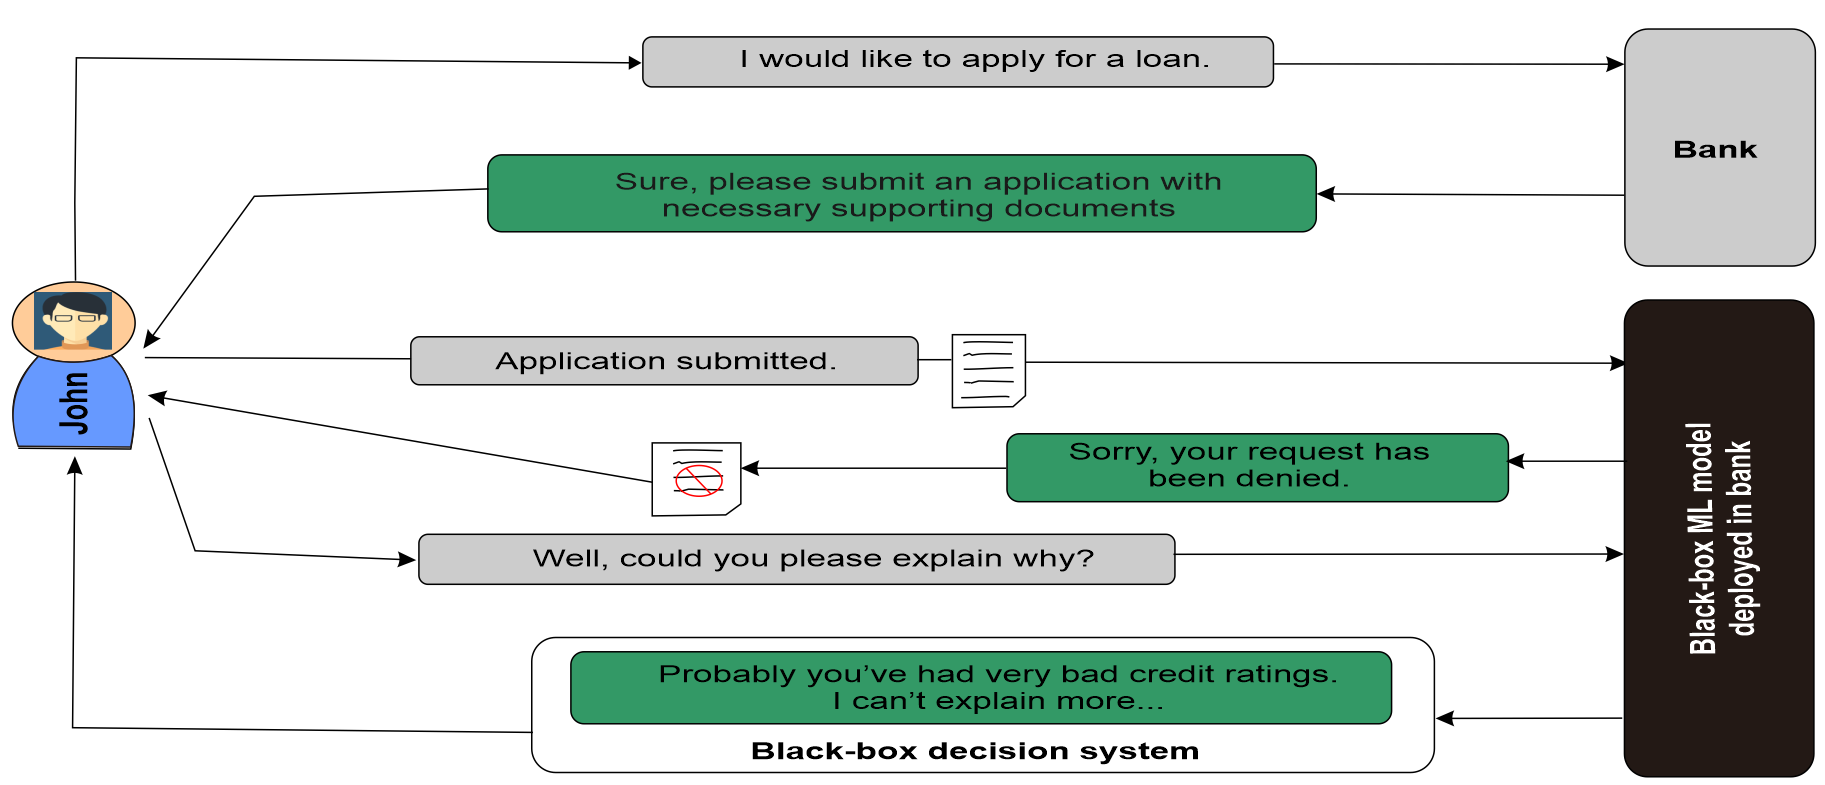
\includegraphics[scale=0.7]{images/loan.png}
	\caption{A black-box DSS cannot explain why a customer's loan application was rejected}
    \label{fig:model_bbm1}
    \vspace{-2mm}
\end{figure*}

\hspace*{3.5mm} Let's assume a simple example of a man named John, who is a typical bank customer. Suppose John applies for a credit~(loan) from a bank.
Then the bank, based on, John's marital status, age, housing, current job status and monthly salary, credit rating history, existing loan, credit amount, duration, etc. will decide if his application will be approved. Suppose, the bank using a ML model, rejected his application. When he asked the lender why it was the case, they should be able to explain the reason why his application was rejected. For example, a minimal explanation could be `\textit{`your application has been rejected, because you had bad credit rating history"}. Although, coming up with such a decision based on a single factor would not make such ML-based credit model necessarily trustworthy and explainable.
However, without rigorous explainability, banks are not able to provide applicants with an adverse action notice such details why they were rejected~\cite{hall2020responsible}. Additionally, they should provide additional information they can use to improve their credit profiles and successfully obtain credit in the future~\cite{hall2020responsible}. 

\hspace*{3.5mm} On the other hand, a linear ML model can make the problem easily interpretable, as long as only a few variables are involved. Suppose we are classifying John as likely to repay or not. Then the minimum information will be used by the ML model is John's annual income and the amount he wants to borrow. We can assume the training data will accompany the outcome. Plotting the training samples will most likely expose that people who repay tend to earn a lot and borrow a little. We can draw a straight line to separate repayers and non-repayers. We can then simply build a linear model keeping in our mind the objective ``is the applicant above or below the line?" Since the predicted repayment probability is a linear function of income and amount, calculating the probability of repayment is trivial: 

\vspace{-2mm}
\begin{align}
    p(r) = A \times income + B \times amount
\end{align}

\hspace*{3.5mm} where $p(r)$ is the probability of repayment, coefficients $A$ and $B$ are two numbers. Such a linear model is inherently interpretable, given that $A$ or $B$ is just a number, and not a function. So, we can trivially set their respective weights and check whether it is positive. Then we can calculate if the repayment probability increases with income. This directional behavior not only matches the expectations of the lenders, but also for John. Besides, the mathematical certainty means we can transparently show that there is no hidden behavior or function influencing the behavior of the model. This ensures our trust is high in the model. Subsequently, based on $A$ and $B$, the lander can explain John why they think John is unlikely to repay in more natural language, such as `\textit{`given your income, you are asking to borrow 50,000\$ is too much}. Even a better explanation could be \textit{``your application has been denied because your debt to income ratio is too high. Pay off 20\% of your debt to increase your approval chances"}. 

\hspace*{3.5mm} Since there is a chance that John might get a better job with higher salary and/or his current loan could already be paid, which will increase his chance in subsequent applications. Then it is trivial to explain the decision to the borrower. However, depending upon lender's credit model, there might be hundreds of other variables involved, where the interactions among each of those variables can be variables too. Such interactions should be observed rigorously, by zooming into individual data points. Nevertheless, since often the relation might not be linear as we thought, they might not be even linearly separable. Subsequently, a linear or tree-based model might not be able to model the relationship. We might even need a complex model such as neural networks, ending up higher accuracy, but less interpretable.  

\subsection{Impacts of black-box DSS in healthcare}
In healthcare, one of the most common applications of traditional ML is precision medicine, e.g., predicting what treatment protocols are likely to succeed on a patient based on patient phenotype, demography, and the treatment contexts~\cite{davenport2019potential}. Recently, AI-guided DSS that used in healthcare is increasingly been applied and adopted in clinical diagnosis, treatment recommendations, patient engagement, and administrative activities in clinical setting~\cite{deepmindhealth}. Even there are many instances, where AI is already outperforming healthcare tasks. AI-guided system is outperforming radiologists at spotting malignant tumours, model the progression, and treatment of cancerous conditions~\cite{deepmindhealth}. Besides, AI is guiding researchers in how to construct cohorts for costly clinical trials~\cite{davenport2019potential}. 

\begin{figure*}
	\centering
	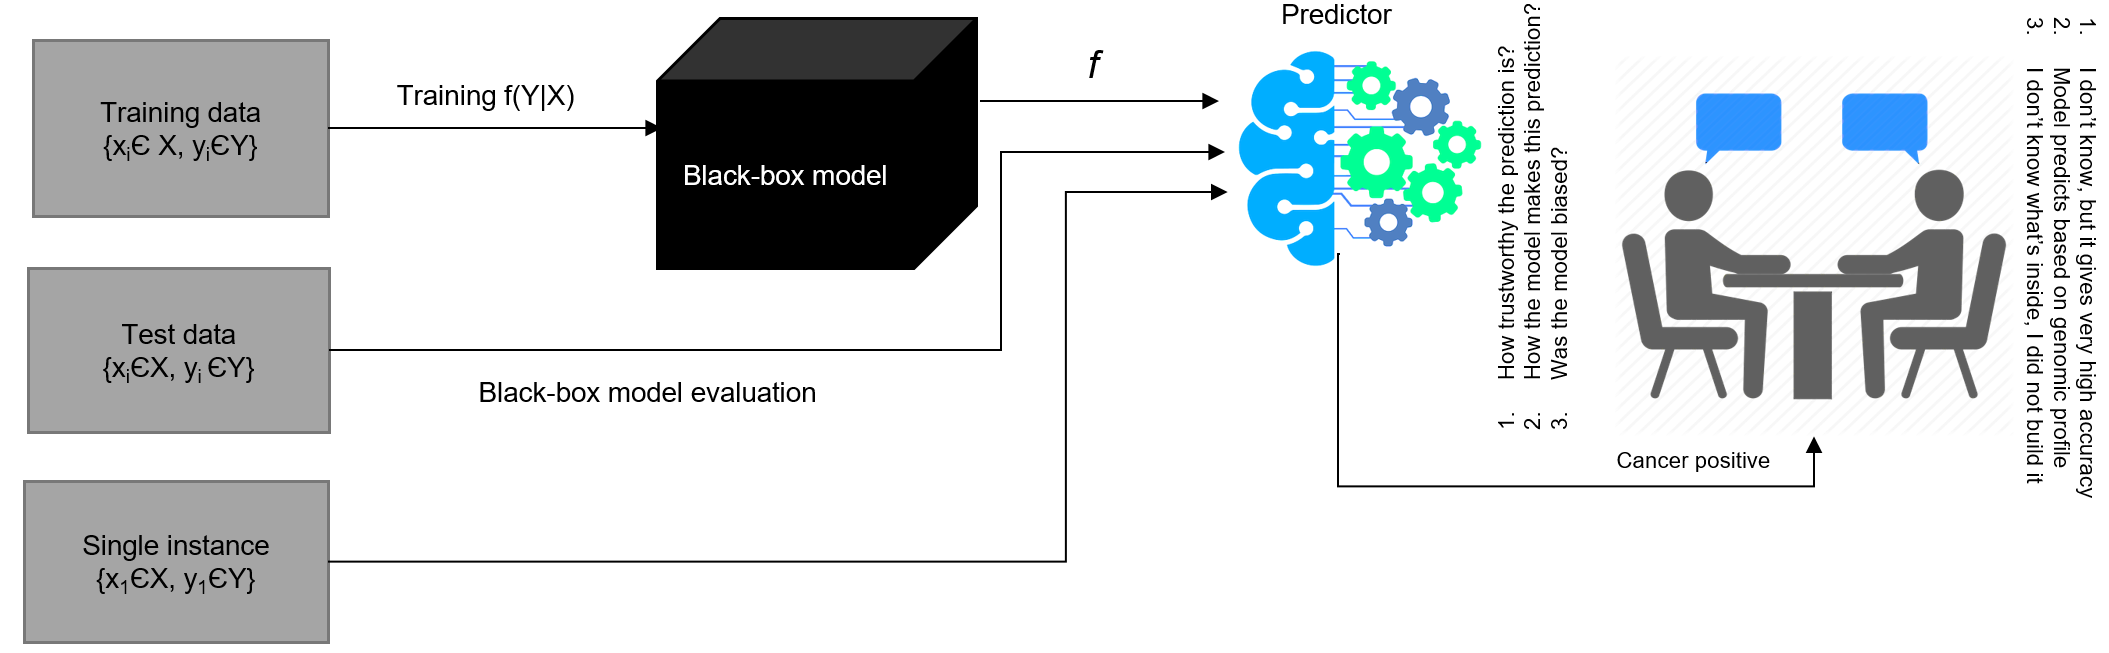
\includegraphics[scale=0.6]{images/bbm.png}
	\caption{A `black-box' model cannot trace back decisions to inputs, i.e., how and why an input is mapped to a output, and vice versa}
    \label{fig:model_bbm2}
    \vspace{-2mm}
\end{figure*}

\hspace*{3.5mm} A more concrete example of using AI-guided DSS in healthcare is carcinogenesis. Cancer has been characterized as a heterogeneous disease consisting of many different types and subtypes, making it is one of the deadliest diseases to treat. Diagnosis and prognosis for specific cancer types is not straightforward. For example, diagnosis of a breast cancer patient depends on several distinct molecular subtypes and multiple factors involved, such as estrogen receptor, progesterone receptor, and human epidermal growth factor receptor. %, providing AI-based diagnoses might not be accurate solely based on CNVs. 
This requires using multimodal features based on DNA methylation, gene expression, miRNA expression, and CNVs data by creating a multiplatform network to support each data type, where the DSS based on genomics data from different cohorts will be more reliable. Subsequently, an early diagnosis of cancer, by classifying cancer patients into high or low risk groups have become essential in cancer research, as it can facilitate the subsequent clinical management of patients~\cite{kourou2015machine}.  
\subsection{Legal aspects}
Given the rapid advances in AI in for healthcare imaging analysis, it seems most radiology and pathology images will be examined at some point by a AI-guided machine. Besides, the day when such AI-guided machines take life decisions for humans is not very far ahead. Consequently, the opaqueness raises numerous legal, ethical, and practical concerns, transparency and accountability in AI-based systems have to ensure. So, if we cannot see how the predictions were made, we cannot know what impact will happen on human lives. Black-box and opaque ML-based credit models can have legal consequences for the lenders. The legal landscape is complex and fast-moving across countries, such as the Equal Credit Opportunity Act and Fair Credit Reporting Act~\cite{act2009fair}. In particular, section 609(f)(1) of the Fair Credit Reporting Act %Nevertheless, failure to do so accurately can result in large fines and/or a suspension of banking license. %Noncompliance is perhaps the most vital reason that lenders have been cautious to adopt machine learning for credit scoring and underwriting.
requires that consumers be provided ``all of the key factors that adversely affected the credit score of the consumer in the model used, the total number of which shall not exceed 4". This enforces lenders to be able to explain the models they use to approve and deny credit applicants. 

\hspace*{3.5mm} The General Data Protection Regulation~(GDPR)~\cite{kaminski2019right} by the European Parliament enforces that individuals should be able to obtain explanations of the decisions made from their data by automated processing, and to challenge the decision. Article 22 states that individuals ``have the right not to be subject to a decision based solely on automated processing" and ``whenever human subjects have their lives significantly impacted by an automatic decision-making machine, the human subject has the right to know why the decision is made"- called `right to explanation', which prohibits the use of ML for automated decisions unless a clear explanation of the logic used to make each decision is well explained. 

%\subsection{Issues with existing interpretable models}
%we don't fully understand how and which factors tend a model to make a prediction right and why it will fail in certain cases
%\Cref{fig:chapter_2_wf} outlines the workflow of the proposed approach to make the model explainable. 

\section{Thesis Goal} \label{thesis_goal}
%Although these models have shown tremendous success in exhibiting high confidence, they are mostly perceived as `black box' methods because of a lack of understanding of their internal functioning. 
Although, not every prediction made by an ML algorithm needs an explanation~\cite{stiglic2020interpretability}, in many cases, ML models itself have to be interpretable enough to ensure that the decisions made by the system is not only accurate, but also trustworthy~\cite{mehrabi2019survey}. 
Coming back to our cancer diagnosis case study. Current cancer typing methods focused on employing ML approaches and using mixed data types to handle the high dimensionality and heterogeneity. However, since predicting cancer types and providing explanation are two of our desired objectives, someone might ask why don't we simply use interpretable models? 
%Eventhough, they perform well, but lack the capability of explain the diagnoses decisions. 
It is well-known that interpretable models and their inner working mechanism are simple. However, such a simple model lacks the capacity and flexibility to capture complex relations and interactions between high dimensional genomic data. In principle, except for the linear and tree-based models, DNN models are perceived mostly as `black box'. Hence often we don't fully understand how and which factors tend the model itself to reach a diagnosis decision, e.g., prediction. % right and why it will fail in certain cases methods as w of their not well-understood internal functioning. Often, . These are serious drawbacks.

\iffalse
\begin{figure}[h]
	\centering
		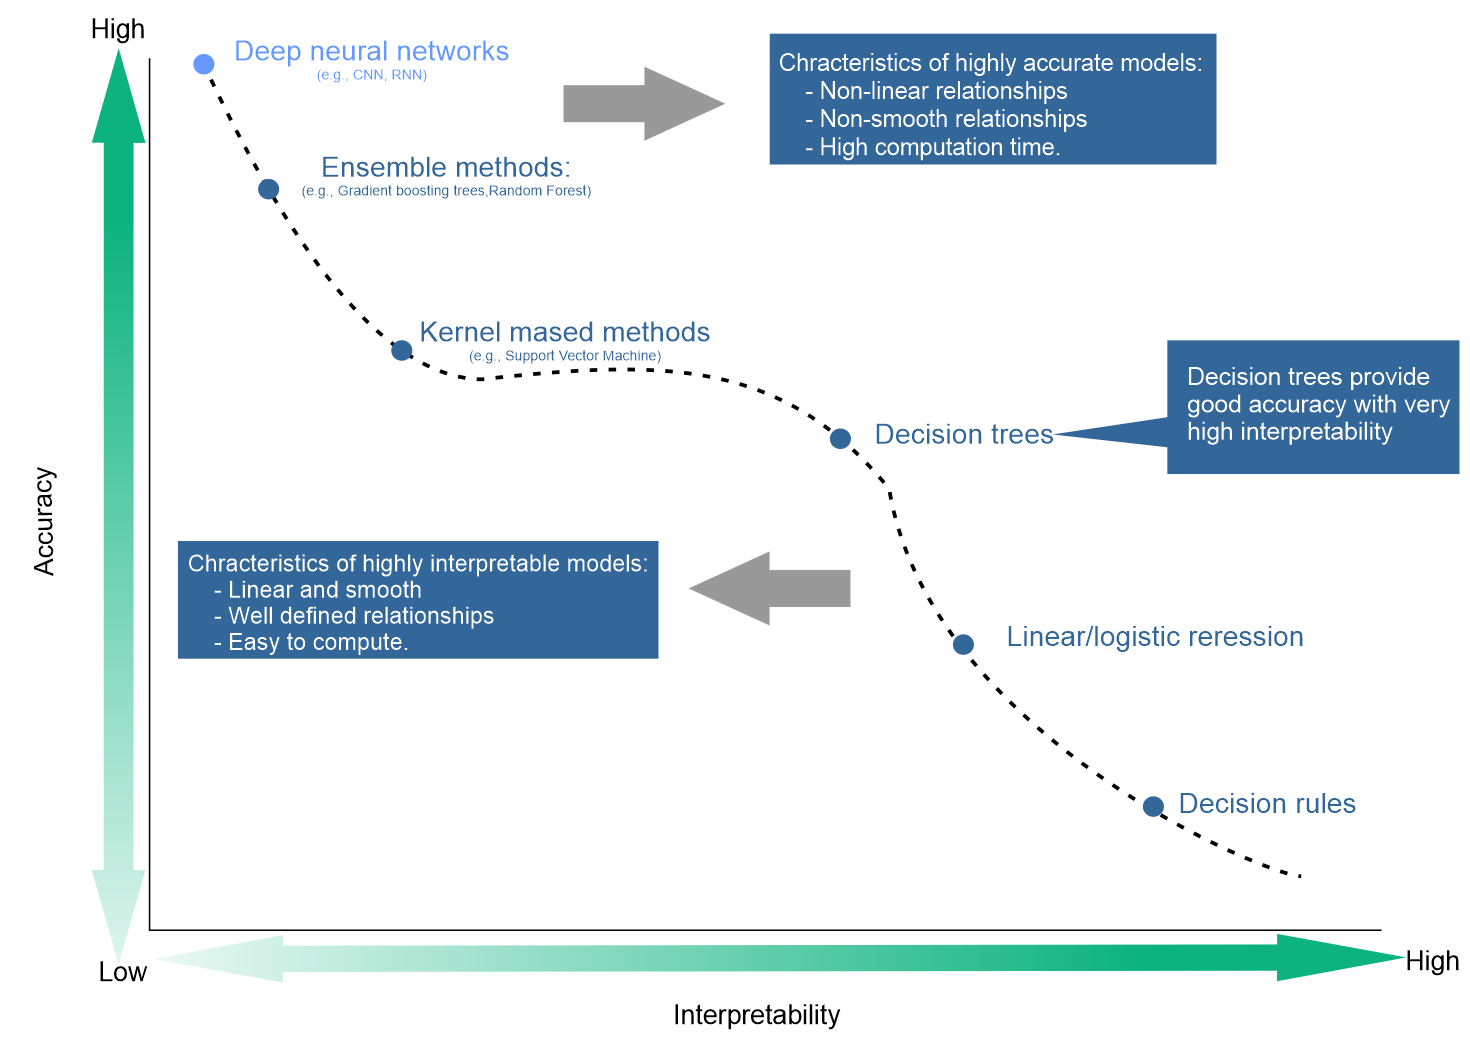
\includegraphics[width=0.7\linewidth,height=70mm]{images/acc_vs_xai.png}
		\caption{The accuracy vs. interpretability trade-off}
        \label{fig:acc_vs_xai}
\end{figure}
\fi

\begin{figure*}
	\centering
	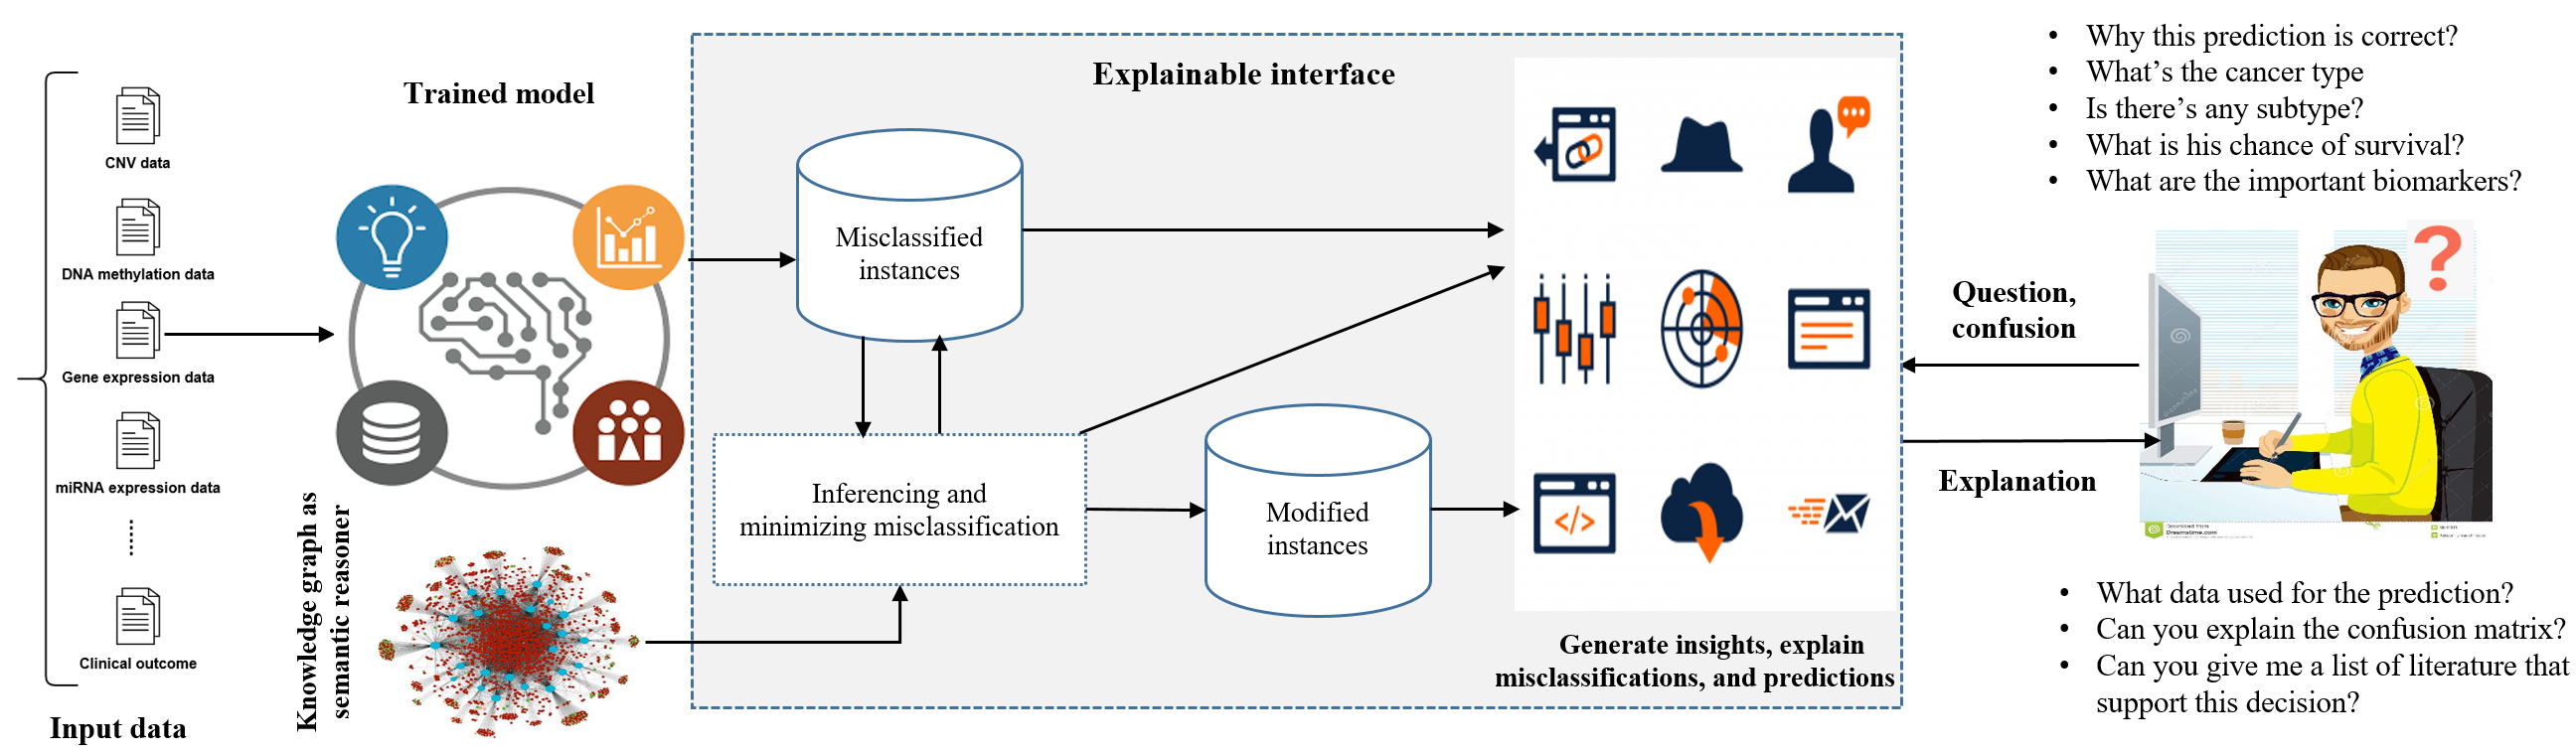
\includegraphics[scale=0.55]{images/xai_interface.png}
	\caption{An explainable DSS is capable to answer ``what", ``why", ``how", and ``where" type of questions}
    \label{fig:model_bbm3}
    \vspace{-2mm}
\end{figure*}

%Higher interpretability of an ML model means easier comprehension and explanation of future predictions for end-users. 
\hspace*{3.5mm} This evolves a fundamental trade-off between accuracy and interpretability: the more interpretable a model is, the less accurate it is. In other words, the most accurate ML models are the least interpretable. %, as shown in \cref{fig:acc_vs_xai}. 
Knowing the cancer type and identifying most relevant biomarkers are the prerequisites for an oncologist to recommend more accurate treatments and drug repositioning. The latter only can be achieved with meaningful explanations, which helps healthcare experts to make reasonable and data-driven decisions to provide personalized diagnosis or treatment decisions that can lead to higher quality of service in healthcare~\cite{stiglic2020interpretability}. Based on a model that is both highly interpretable and accurate, developing an explainable DSS to improve the transparency and trustworthiness for cancer diagnosis is the main goal of this thesis, such that the DSS will be able to: 

%\vspace{-2mm}
\begin{enumerate}[noitemsep]
    \item Generate accurate and trustworthy predictions in a transparent way
    \item Provide human-interpretable explanations of the decisions made
    \item Identify and explain misclassified instances, 
    \item Validate the decisions based on domain-knowledge from a knowledge base~(KB)
    \item Produce and help disseminate new knowledge. 
\end{enumerate}
%\vspace{-2mm}

\hspace*{3.5mm} Since ML ecosystem can be aligned with different questions about ``what", ``why", ``how", and ``where" a computer program is carried out~\cite{zednik2019solving}, knowing answers to these will assist the doctors to answer different types of questions asked by the end users during the diagnosis process. For example, cancer types can be identified by learning similarities from patients genomic profiles.   

\section{Problem Statement} \label{problem_challenges}
The problem of classifying the patients is grouping into a specific cancer types based on their unimodal or multimodal genomic profiles. In other words, the cancer typing method can be formulated as a prediction in a multi-class classification setting, where cancer types and subtypes can be defined as follows: % in the context of a DSS for cancer diagnosis: 

\begin{itemize}[noitemsep]
    \item \textbf{Cancer types} - cancers are named for the area in which they begin and the type of cell they are made of, even if they spread to other parts of the body, e.g., a cancer that begins in the lungs and spreads to the liver is still called lung cancer~\cite{19Cruz}. 
    \item \textbf{Cancer subtypes} - it describes the smaller groups that a type of cancer can be divided into, based on certain characteristics of the cancer cells.  %Besides, there are several clinical terms used to describe certain types of cancer\footnote{\url{https://www.healthline.com/health/cancer\#types}}.
\end{itemize}

\hspace*{3.5mm} Often decision support systems have to provide decision based on different types of data. In such case, each input type can can be considered as individual input modalities. On the other hand, multimodality refers to the way to integrate multiple such input modalities~\cite{mmsurvey}. Let $X$ = $\left(x_{1}, x_{2}, \ldots, x_{n}\right)$ be a genomic dataset of $n$ samples, where a sample $x_i$ composed of $m$ independent real-valued genes $G$ = $\left(g_{1}, g_{2}, \ldots, g_{m}\right)$. %, $X \in \mathbb{R}^{D}$, and $G \in \mathbb{R}^{D}$.
In other words, sample $x_i$ consists of a set of $m$ real-valued attribute-value pairs $\left(a_{i}, v_{i}\right)$, where $a_i$ is a feature and $v_i$ is its value.
%, such that both $a_{i}$ and $v_i \in \mathbb{R}^{D}$. 
To solve the multiclass-classification problem, first we train a DNN architecture and generate a robust `black-box' model, instead of relying on interpretable models. 

\hspace*{3.5mm} However, in case of multiple $k$ input modalities, 
%it will contribute as another input modality towards multimodality, where to generate the modality specific latent representation of the input modalities. 
i.e., multimodal genomic dataset $D=\{X_1, X_2,..., X_k\}$, we  consider classifying an individual $x_i$ into a specific cancer type by learning the modality specific latent representation based on his or her genomic profile. %, where %$x_k \in \mathbb{R}^{D}$,
%where $X_k$ = ${\mathbf{\{x_1,x_2,..., x_n}}\}$ is represent an individual input modality. 
Since each modality is comprising very high dimensional genomic data, we embedded each input modality $x_i$ into lower dimensional feature space instead of classifying them using their original representation. In other words, using learned representation from individual modalities, we train a `black-box' DNN model, as shown in \cref{fig:chapter_2_wf}, such that we transform each input modality $X$ with a nonlinear mapping $f_{\theta}: x_i \rightarrow z_i$, where $\theta$ are learnable parameters and $z_i \in \mathbb{R}^{K}$ is the learned embedding in which $K \ll D$. 

\begin{figure*}[h]
	\centering
		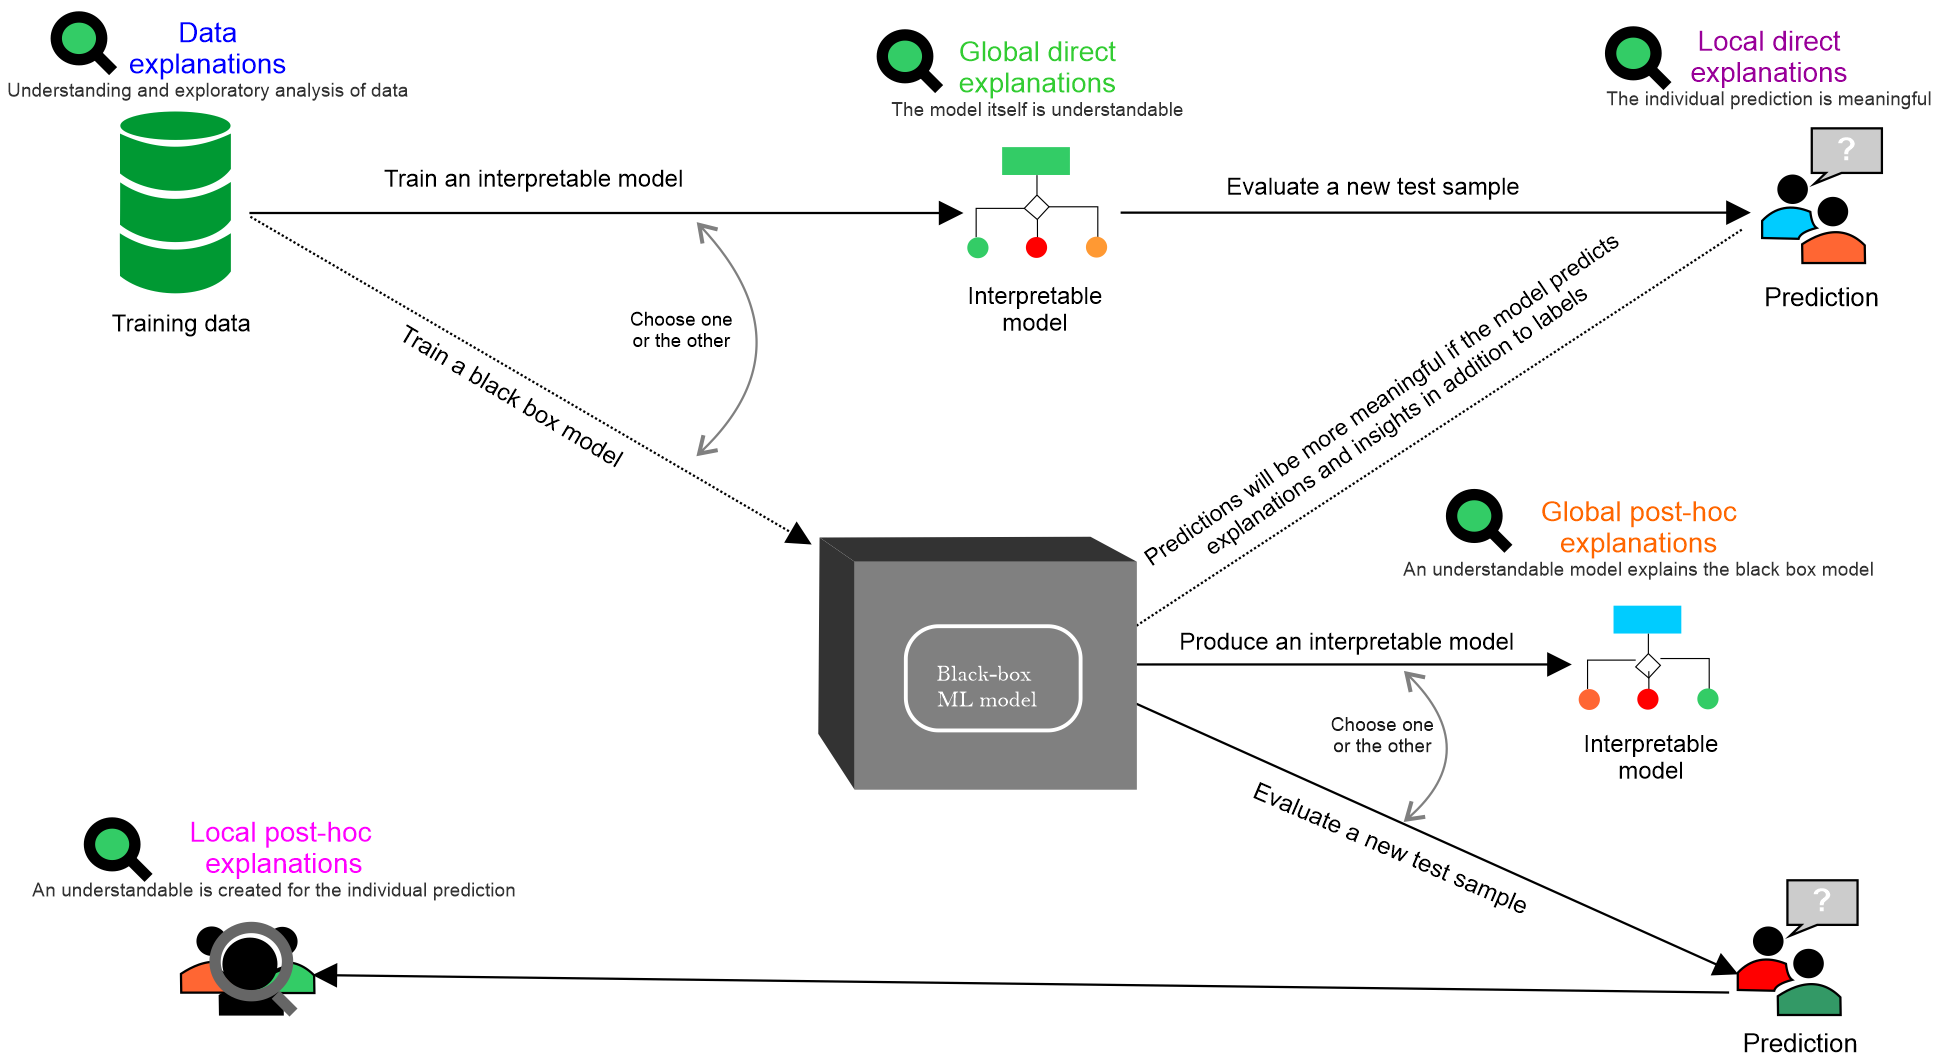
\includegraphics[scale=0.6]{images/g_t_l_xai.png}
		\caption{Workflow of the proposed approach to make the model explainable}
        \label{fig:chapter_2_wf}
\end{figure*}

\hspace*{3.5mm} To parametrize $f_{\theta}$, we employ neural network-based representation learning~(e.g., autoencoders) due to their function approximation properties and feature learning capabilities~\cite{xie2016unsupervised} from genomic data. The input is fed into the encoder %$f_\theta$ 
to generate a modality specific latent representation $z$. Latent representation is then fed into the decoder module to reconstruct ${x}_{i}^{\prime}$, similar to the original input $x_i$. The parameters of the modality specific network are then trained to minimize the error between the decoder’s output and the input signal. The latent representations of all modalities are then concatenated into a single representation $Z$ = $h_{i,j} \in \mathbb{R}^{D}$. A classifier $f$ then maps a data point $x_i$ to an output $f(x_i) \mapsto y_i$ in the embedded space $Z$. Since neither the decision made by $f$ be traced back to the inputs, nor it is clear why the outputs are transformed the way they are, it is arguable to treat $f$ a `black-box' model, where the concept of 'black-box' and `white-box' can be described as follows:   

\begin{itemize}[noitemsep]
    \item \textbf{Black-box model} - an ML model $f$ is considered black-box if the model parameters and network architectures are hidden from  end-users~\cite{das2020opportunities}. 
    \item \textbf{White-box model} - an ML model $f$ is white-box if its parameters $\boldsymbol{\theta}$ and architecture are known to the end users, and users have sufficient know-how and why it provides decision/prediction~\cite{das2020opportunities}.  
\end{itemize}

\hspace*{3.5mm} By emphasizing specific characteristics of a patient that represents the characteristics of a smaller group of cancer patients such as breast cancer, yet different in other patients~(rather than all the patients in a dataset). By embedding both local and global interpretability logic, we make ``black-box" model $f$ interpretable in a post-hoc manner. We now introduce the concept of `interpretability', `local interpretability', and `global interpretability' of ML systems: 

\begin{itemize}[noitemsep]
    \item \textbf{Interpretability} - is the degree to which a human can understand the cause of a decision.
    \item \textbf{Global interpretability} - how does the trained model make predictions~\cite{molnar2019interpretable}? It enables a model to explain conditional interactions between dependent and independent variables, i.e., it involves explaining the overall relationship between features and labels.
    \item \textbf{Local interpretability} - why did the model make a certain prediction for an instance~\cite{molnar2019interpretable}? It enables an explainable model to explain the conditional interaction between dependent and single prediction, i.e., focuses on explaining the prediction of an individual instance. 
\end{itemize}

\hspace*{3.5mm} We explain a data point $x_i$ using an explanation function $g$. Local interpretability refers to an explanation giving reasoning why the model $f$ has predicted $f(x_i)$ for a data point $x_i$, during inferencing. Since providing human-level interpretability by ``zooming in" individual predictions makes the explanation more evident~\cite{ribeiro2018anchors}, we answer the following questions based on local explanation methods: 

\begin{itemize}[noitemsep]
    \item Which feature $x_i \in X$ was most important for a certain prediction with $f$? 
    \item Which training data point $x_i \in X$ was most important to $f(x_i)$? 
    \item What minimal change is necessary to input $x$ to change the output $f(x_i)$?
\end{itemize}

\hspace*{3.5mm} As the global interpretability signifies the overall transparency of a model on an abstract level, a surrogate model is often used to explain it's global behaviour by approximating the behaviour of the original  model, where the `algorithmic transparency' and `model surrogate strategy' can be described as: 

\begin{itemize}[noitemsep]
    \item {\textbf{Algorithmic transparency}} - is the principle that the factors that influence the decisions made by algorithms should be visible, or transparent, to the people who use, regulate, and are affected by systems that employ those algorithms.It also signifies how a learning algorithm learns a model from the data by mapping relations to make prediction for unknown sample.
    \item \textbf{Model surrogation} - a model interpretation strategies, which involve training an inherently interpretable model using the same data to approximate the predictions of the `black-box' model. 
\end{itemize}

\hspace*{3.5mm} Using an oracle or a surrogate model, we answer following questions with global explanation methods: 

\begin{itemize}[noitemsep]
    \item What feature(s) $x_i \in X$ are most important across predictions for $f$?
    \item What training data points $x_i \in X$ are most important to $f(x_i)$? 
    \item What minimal change is necessary to input sample $x_i$ to change the output $f(x_i)$?
\end{itemize}

\begin{sidewaysfigure*}
	\centering
	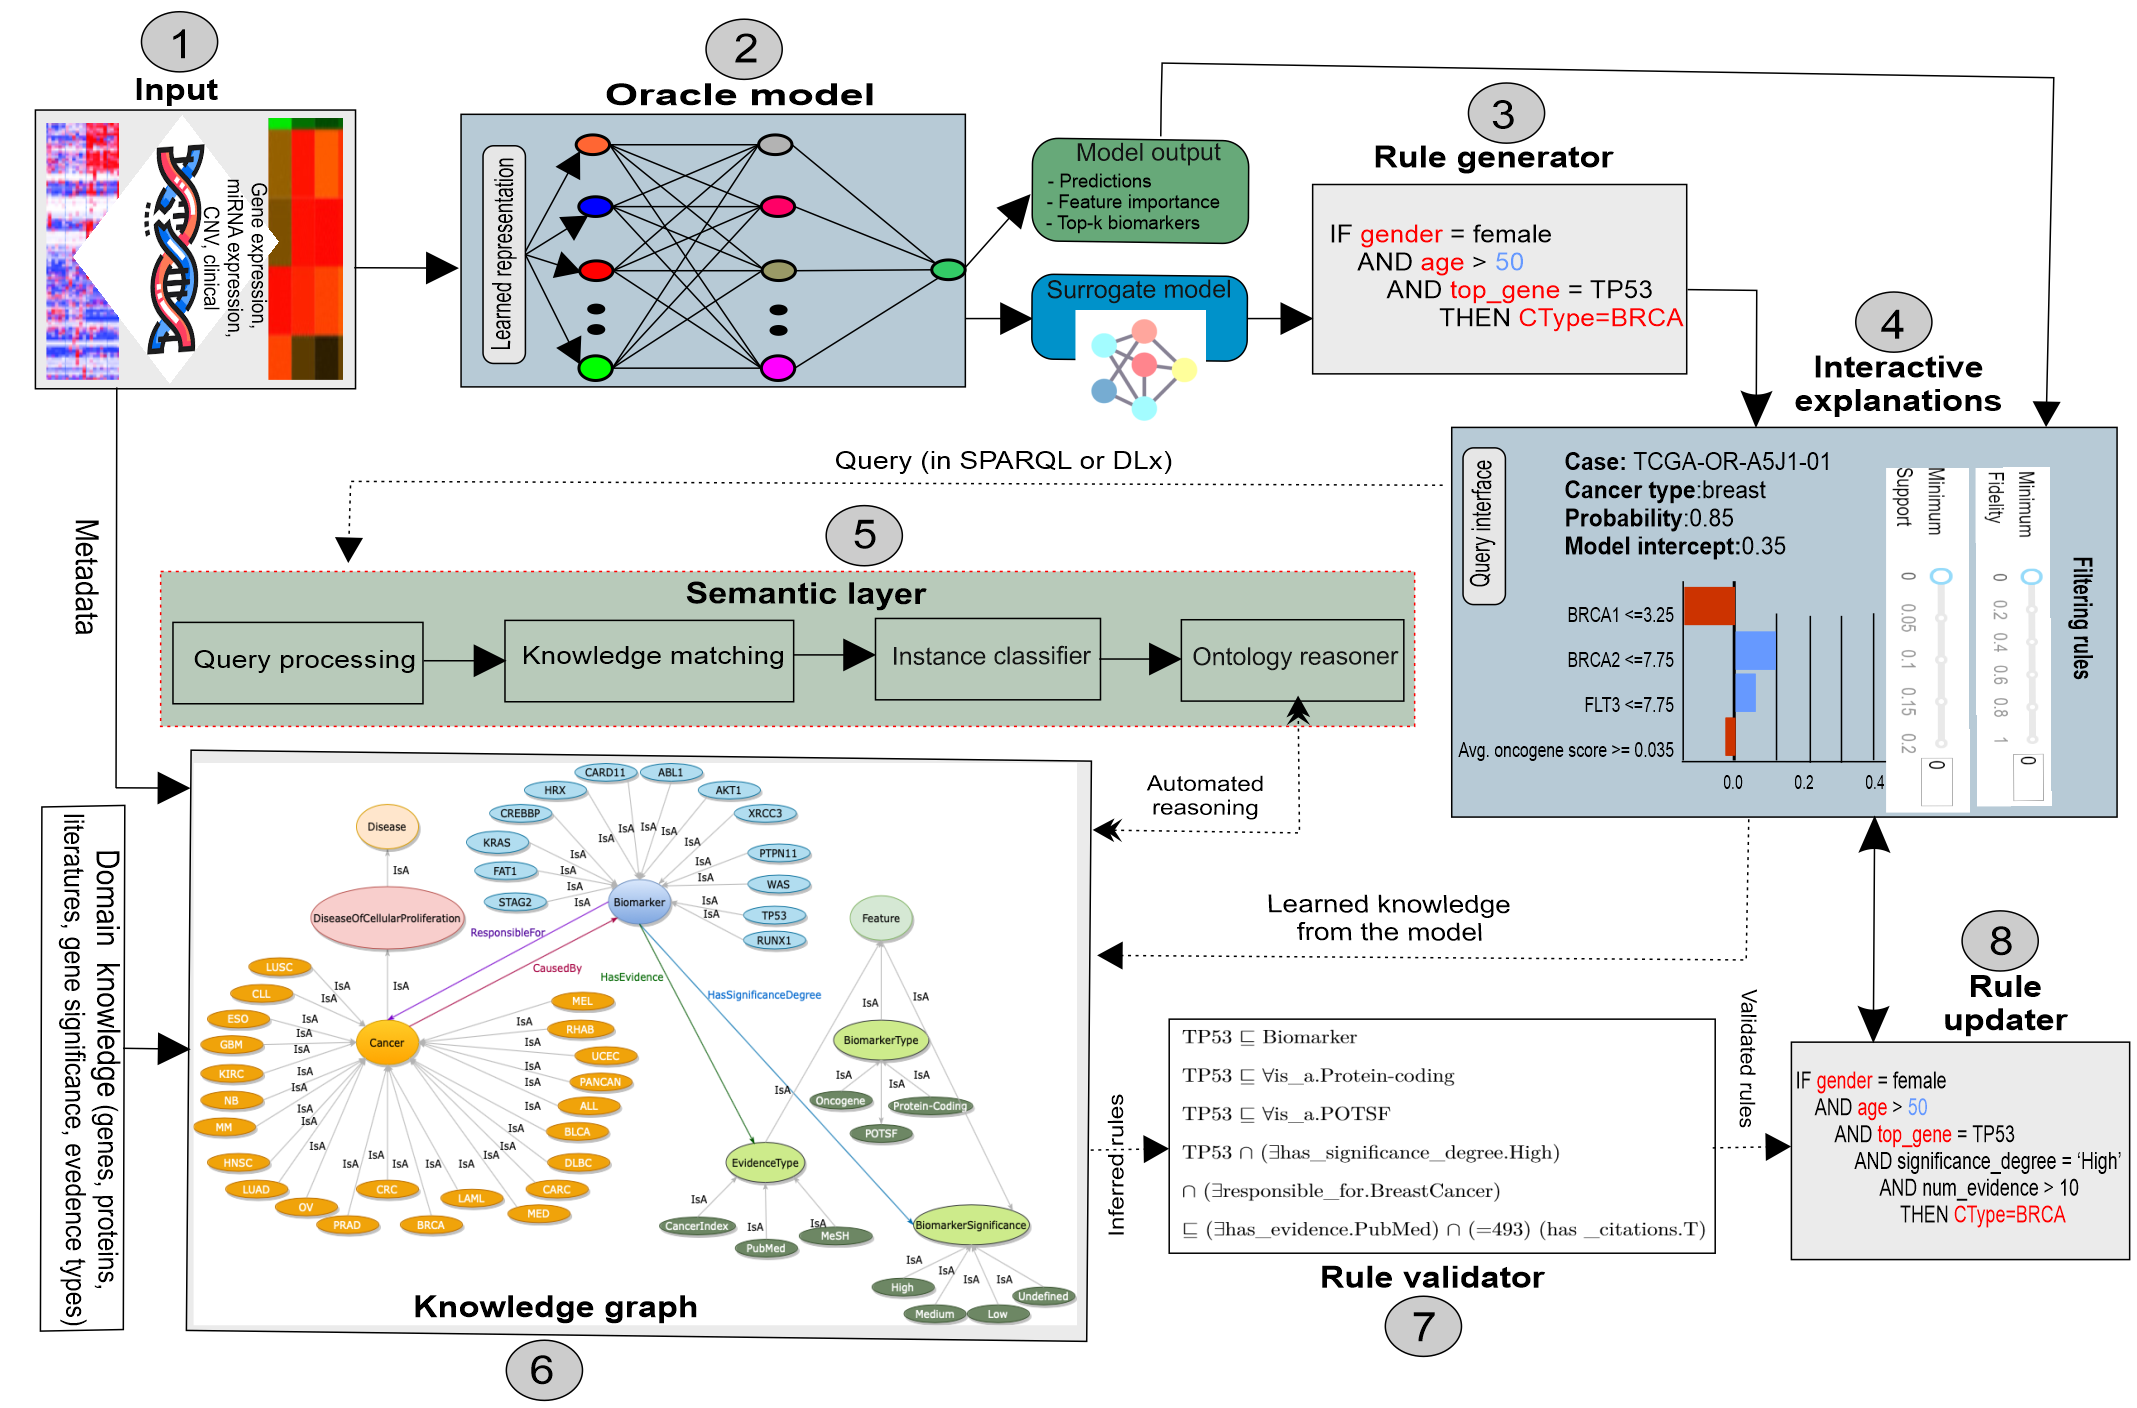
\includegraphics[scale=0.8]{images/reasoning_wf.png}
    \caption{Workflow for improving the explainability and transparency of a clinical DSS}
	\label{fig:wf_overall_approach}
\end{sidewaysfigure*}

\hspace*{3.5mm} Further, we validate our findings through functional analysis to make sure the selected genes are biologically trustworthy for the corresponding tumor types. In particular, based on annotations from the TumorPortal\footnote{
TumorPortal provides knowledge and annotations about genes, cancers, and DNA mutations, link-\url{www.tumorportal.org}}, we will validate our findings to ensure biological relevance. \Cref{fig:wf_overall_approach} depicts the workflow of the proposed approach for making the DSS transparent and explainable for cancer diagnosis. As depicted, we train several unimodal and multimodal DNN architectures on genomics data and clinical outcome to learn high-level abstract features. Neural ensemble method, which is more effective than structures solely based on a single model is then employed to get the most stable model from multiple model snapshots. Subsequently, we identify cancer-specific driver genes and provide explanations of the predictions based on decision rules focusing both local and global interpretability. 

\hspace*{3.5mm} To improve adversarial robustness, we introduce different adversarial attacks on the models and perform adversarial training to adversaries and behaves as intended in real-life scenario, a is necessary. As a part of the symbolic reasoning~(SR), we develop a domain-specific knowledge graph~(KG) by integrating knowledge and facts about cancer from external sources, which provides the foundation of the semantic layer. A semantic reasoner that characterizes and learns hierarchical relations from the KG, is used to provide the reasoning about diagnosis decision. 
Finally, decision rules are updated by combining reasoning and predictions to make the clinical diagnosis. The role of a reasoner would be answering queries based on the prediction whose answers will be derived from the symbolic rules stored in the KG.  

\hspace*{3.5mm} On a serious note on usability of an XAI system, interactive ML adds the component of human expertise to AI/ML processes by enabling them to re-enact and retrace AI/ML results\footnote{For example, let them check it for it's user-friendliness, effectiveness, and plausibility}~\cite{holzinger2020measuring}. This requires human–AI interfaces for the DSS. In order to build effective and efficient interactive human–AI interfaces we have to deal with the question of how to evaluate the quality of explanations given by an explainable AI system~\cite{holzinger2020measuring}. 

\section{Hypotheses and Research Questions} \label{hypotheses}
To improve the transparency and explainability of a DSS and to disseminate biological knowledge about carcinogenics, we attempt to solve the research questions that are driven by several hypotheses.  

\subsection{Research questions}
This thesis attempts to solve the following 5 research questions on which the DSS is built upon:  

\vspace{-2mm}
\begin{itemize}[noitemsep]
    \item \textbf{RQ1}: \textit{How can multimodal data be more effective than unimodal data to provide accurate decision?} As mentioned earlier, multiple factors are involved in cancer diagnosis, genomics data such as GE, miRNA expression, copy numbers, and clinical outcome have to use together to build a more efficient model to accurately predict the outcome of a diagnosis decision.  
    \item \textbf{RQ2}: \textit{How to identify relevant features or factors for a certain decision?} Identification of important biomarkers that contributed most~(i.e., some of the features have a higher impact than others), which facilitates the identification and validation of the presence of cancer and also help determine its stage, subtype, and whether they will respond to therapy. Cancer biomarkers are also of potential therapeutic targets and a key in sequence-specific gene silencing therapy against cancer by selectively silencing aberrantly activated oncogenes.  
    \item \textbf{RQ3}: \textit{How to provide human-understandable interpretations of the decisions using decision rules?} Decision rules are more effective at providing intuitive explanations. Using a set of rules, it is possible to explain a decision directly to humans with the ability to look up the reason for a decision. 
    %\textbf{${RQ}_5$}: How to generate human-interpretable decision rules to provide transparent cancer diagnosis? \\
    \item \textbf{RQ4}: \textit{How to disseminate and validate embedded domain knowledge in the model?} An explainable ML model can not only provide predictions, but also insights about top biomarkers, gene correlations, biomarkers types, etc. These help to understand the mechanisms of carcinogenesis, to be further validated with expert domain knowledge. 
    \item \textbf{RQ5}: \textit{How to score a `black-box' model on transparency?} Knowing the answer to this question will enable us why did the model behave in a certain way? 
\end{itemize}
\vspace{-2mm}

\subsection{Hypotheses}
%To reach the goal, we solve the above research questions, which are driven by the hypotheses.
This thesis makes the following 8 hypotheses, which will lead towards potential solutions to the research questions mentioned above in case they are confirmed:

%\vspace{-2mm}
\begin{itemize}[noitemsep]
    \item \textbf{H1}: Stacking- and neural representation learning can be very effective at handling high dimensional genomic data and to extract most abstract features through a hierarchical learning process. 
    \item \textbf{H2}: A neural ensemble method, combining several deep architectures, can be more effective than structures solely based on a single model by reducing the generalization error. 
	\item \textbf{H3}: Multimodal genomics data and clinical outcomes can be used to train a multimodal neural network architecture to provide more accurate clinical diagnostic decision. 
    \item \textbf{H4}: Since genomics data is high dimensional, embedding them into 2D raw images can help locate significant~(i.e, most and least) biomarkers. 
    \item \textbf{H5}: An interpretable `black-box' model can answer why and how a certain diagnosis decision is made by highlighting most significant~(i.e, most and least) biomarkers for clinical validation. 
    \item \textbf{H6}: The attention mechanism can be applied on encoder's bottleneck layer to generate attention weight vector, which can be decomposed to compute modality specific feature attributions. 
    \item \textbf{H7}: A surrogate model can be used to approximate the predictions~(embedded knowledge) of a partially `white-box' model and generate decision rules for diagnosis decisions. 
    \item \textbf{H8}: Ontological reasoning can characterize errors~(in diagnosis decision) w.r.t hierarchical relations between entities in the KB that helps in the decision making process.
    \item \textbf{H9}: Fair decision rules can be deduced by combining model predictions and symbolic reasoning. 
\end{itemize}
%\vspace{-2mm}

\hspace*{3.5mm} \Cref{fig:wf_overall_approach} outlines workflow of the  approach to improve the transparency and explainability of a DSS. 

\section{Key Contributions} \label{contributions}
The main contributions of this thesis can be summarized as follows:

\begin{itemize}[noitemsep]
    \item A labelled multimodal genomics data is prepared for cancer type prediction, which can be used to develop an explainable DSS.  
    \item Several robust neural network architectures were trained in which different interpretable methods and explainable logic are embedded. These approach enhance the capability of the learning algorithm to identify most significant biomarkers and provide class-specific explanations giving the top-k and common genes across cancer types. 
    \item Adversarial training is performed to make the explainable model robust against different types of attacks, such as content moderation and out-of-distribution attacks. 
    \item A novel method for generating decision rules is proposed for cancer diagnosis, by combing model prediction, top biomarkers, and reasoning based on symbolic reasoning. 
    \item Both proactive and reactive measures were taken to make the diagnosis decision trustworthy by mitigating different types of bias. 
    \item A user-friendly interface is developed\footnote{Can be accessed at: \url{http://xai.fit.fraunhofer.de:5000/cancer/}} to leverage more human-interpretable explanations, covering both global and local explanations of the diagnosis made. 
    \item Comprehensive evaluations with detailed analyses of outcomes and comparisons with state-of-the-art. 
\end{itemize}

\hspace*{3.5mm} These contributions were disseminated into 3 directions: i) peer-reviewed scientific publications, ii) public talks and presentations, iii) open source contributions. %, e.g., implementations of some approaches presented. %A number of peer-reviewed publications were produced while conducting the work in this thesis. They are mentioned below, and a note is made to their relevant chapters. 

\subsection{Relevant publications}
Above scientific contributions were reflected in a number of peer-reviewed publications. We provide notes to their relevance, where some of these publications help build the foundation of this thesis: 

\begin{enumerate}
	\item {Alokkumar Jha, Yasar Khan, Muntazir Mehdi, \textbf{Md. Rezaul Karim}, Qaiser Mehmood, Achille Zappa, Dietrich Rebholz-Schuhmann, and Ratnesh Sahay, ``Discovering Biomarker and Pathway for Gynecological Cancers", \emph{Journal of Biomedical Semantics}, 8(1), September 2017} 
	
	\textbf{Abstract}: In this paper, we present an approach to link and query different sequencing datasets such as TCGA, COSMIC, REACTOME, KEGG, and GO to indicate risks of different cancer types. We analyse the tissue expression of genes, CNV, somatic mutation, and promoter methylation to identify associated pathways and find novel biomarkers. 
	
	\textbf{Relevance}: this publication helps provide basic understanding of carcinogenics and different types of genomics data needed to be analyse towards biomarker discovery in \cref{chapter:introduction} and \cref{chapter:preli}. While working on the paper, I get acquainted with cancer genomic data for the first time. I contributed in the generation of 5* linked data that were lately integrated to form a large-scale knowledge graphs. 
	
	\textbf{Link}:~\url{https://jbiomedsem.biomedcentral.com/articles/10.1186/s13326-017-0146-9}
	
	\item \textbf{Md. Rezaul Karim}, Stefan Decker, Oya Beyan, ``Cancer Risk and Type Prediction Based on Copy NumberVariations with LSTM and Deep Belief Networks", \emph{Proc. of Artificial Intelligence International Conference (A2IC'2018)}, November 21-23, Barcelona, Spain. 
	
	\textbf{Abstract}: In this paper, we apply DL methods to identify cancer and tumor types using CNVs extracted from cancer genomics data from TCGA. We identify and extract CNVs based on long short-term memory~(LSTM) and deep belief networks~(DBN). These were trained using two different representations of CNVs: based on oncogenes and all human genes. Due to lack of sufficient amount of labeled data, we pre-trained the DBN in an unsupervised way then the supervised fine-tuning was carried out using both feed-forward and LSTM networks. 
	
	\textbf{Relevance}: this publication was one of the first attempts to apply DL in cancer types prediction, which motivates us employing more advanced DNN architectures in chapter \ref{chapter:uni_modality}, \ref{chapter:multiodality}, \ref{chapter:xai}, and \ref{chapter:robustness}.
	
	\textbf{Link}:~\url{https://www.premc.org/doc/A2IC2018/A2IC2018_Book_Of_Abstracts.pdf}
	
	\textbf{GitHub}:~\url{https://github.com/rezacsedu/Cancer-Risk-Type-Prediction-CNV-LSTM-DBN}
	
	\item \textbf{Md. Rezaul Karim}, Oya Beyan, Achille Zappa, Ivan G. Costa, Dietrich Rebholz-Schuhmann, Michael Cochez, and Stefan Decker, ``Deep Learning-based Clustering Approaches for Bioinformatics", \emph{Briefings in Bioinformatics}, 02 February, 2020.
	
	\textbf{Abstract}: In this paper, we review state-of-the-art DL-based approaches for cluster analysis that are based on representation learning. We also discussed why and how the representation learning based on different autoencoder architectures are more effective at clustering high dimensional datasets than classic clustering algorithms, covering bioimaging, GE, and biomedical texts. 
	
	\textbf{Relevance}: this publication forms the foundations of representation learning based on variational, LSTM, and convolutional autoencoders used in chapter \ref{chapter:multiodality}, \ref{chapter:xai}, and \ref{chapter:robustness}.

	\textbf{Link}:~\url{https://academic.oup.com/bib/advance-article/doi/10.1093/bib/bbz170/5721075}
	
	\textbf{GitHub}:~\url{https://github.com/rezacsedu/DL_Clustering_Bioinformatics}
	
	\item \textbf{Md. Rezaul Karim}, Michael Cochez, Oya Beyan, Dietrich Rebholz-Schuhmann, and Stefan Decker, ``Convolutional Embedded Networks for Population Scale Clustering and Bio-ancestry Inferencing", \emph{IEEE/ACM Transactions on Computational Biology and Bioinformatics}, 2020.
	
	\textbf{Abstract}: in this paper, we proposed convolutional embedded networks~(CEN) in which we combine two DNN architectures called convolutional embedded clustering~(CEC) and convolutional autoencoder~(CAE) classifier for clustering individuals and predicting geographic ethnicity, respectively, based on genetic variants~(GVs). We employed CAE-based representation learning on GVs from the `1000 genomes' and `Simons genome diversity' projects. This publication forms the foundations of representation learning based on CAE used in \cref{chapter:uni_modality} and \cref{chapter:xai}.

	\textbf{GitHub}:~\url{https://github.com/rezacsedu/Recurrent-Deep-Embedding-Networks}
	
	\item \textbf{Md. Rezaul Karim}, Stefan Decker, Oya Beyan, ``Drug-Drug Interaction Prediction Based on Knowledge Graph Embeddings and Convolutional-LSTM Network", \emph{In Proc. of ACM International Conference on Bioinformatics, Computational Biology, and Health-informatics~(ACM-BCB)}, Niagara Falls, New York, USA, September 7-10, 2019.
	
	\textbf{Abstract}: In this paper, we propose a new approach for predicting drug-drug interactions~(DDI) with Convolutional-LSTM network trained on multiple data sources. For this task we use drug features from DrugBank, PharmGKB, and KEGG drugs, which are integrated using Knowledge Graphs~(KGs). Our evaluations against several baseline models outperforms state-of-the-art approaches. 
	
	\textbf{Relevance}: this publication further motivates us employing Conv-LSTM network in \cref{chapter:uni_modality}.
	
	\textbf{Link}:~\url{https://dl.acm.org/doi/10.1145/3307339.3342161}

	\textbf{GitHub}:~\url{https://github.com/rezacsedu/DDI-prediction-KG-embeddings-Conv-LSTM}
	
	\item \textbf{Md. Rezaul Karim}, Ashiqur Rahman, Stefan Decker, and Oya Beyan, ``A Snapshot Neural Ensemble Method for Cancer Type Prediction based on Copy Number Variations", \emph{Neural Computing and Applications}, 30 November 2019. 
	
	\textbf{Abstract}: in this paper, we used CNVs data covering different cancer types from The Cancer Genome Atlas~(TCGA).We construct two sparse representations of CNVs based on oncogenes and protein-coding genes. Then we train Conv-LSTM and convolutional autoencoder~(CAE) networks using both representations and create snapshots models. While the Conv-LSTM can capture locally and globally important features, CAE can utilize unsupervised pre-training to initialize the weights in the subsequent convolutional layers against the sparsity. Model averaging ensemble~(MAE) is then applied to combine the snapshot models in order to make a single prediction. 
	
	\textbf{Relevance}: this publication further forms the foundation of applying snapshot neural ensemble technique in chapters \ref{chapter:uni_modality} and \ref{chapter:xai}.
	
	\textbf{Link}:~\url{	https://link.springer.com/article/10.1007/s00521-019-04616-9}
	
	\textbf{GitHub}:~\url{https://github.com/rezacsedu/Cancer-type-prediction-CNV_LSTM-CAE} 
	
	\item \textbf{Md. Rezaul Karim}, Stefan Decker, Oya Beyan, ``Prognostically Relevant Subtypes and Survival Prediction for Breast Cancer Based on Multimodal Genomics Data", \emph{IEEE Access}, September 2019.
	
	\textbf{Abstract}: In this paper, a new approach was proposed to analyze multimodal genomics data from TCGA. DNA methylation, GE, and miRNA expression data were used by creating a multiplatform network called multimodal autoencoders~(MAE) classifier to classify breast cancer patients based on their subtypes and survival rates.
	
	\textbf{Relevance}: this publication inspired me to apply MAE technique in \cref{chapter:xai}.
	
	\textbf{Link}:~\url{https://ieeexplore.ieee.org/document/8839793}
	
	\textbf{GitHub}:~\url{https://github.com/rezacsedu/MultimodalAE-BreastCancer}
	
	\item \textbf{Md. Rezaul Karim}, Michael Cochez, Oya Beyan, Stefan Decker, and Christoph Lange-Bever, ``OncoNetExplainer: Explainable Predictions of Cancer Types Based on Gene Expression Data", \emph{In proc. of IEEE International Conference on Bioinformatics and Bioengineering~(BIBE 2019)}.
	
	\textbf{Abstract}: In this paper, we propose a new approach called \emph{OncoNetExplainer} to make explainable predictions of cancer types based on GE data on which we trained CNN and VGG16 networks using Grad-CAM++. We generate class-specific heat maps to identify significant biomarkers and computed feature importance to rank top genes across all the cancer types. Further, we identified top genes, and cancer-specific driver genes using gradient boosted trees and SHapley Additive exPlanations~(SHAP). Findings were validated with the annotations provided by the TumorPortal. 
	
	\textbf{Relevance}: this publication further forms the foundation of applying MAE technique in \cref{chapter:xai}.
	
	\textbf{Link}:~\url{https://ieeexplore.ieee.org/document/8941872}

	\textbf{GitHub}:~\url{https://github.com/rezacsedu/XAI_Cancer_Pred}
\end{enumerate}

%The articles in this dissertation are all related to knowledge evolution. The Venn diagram in fig. 7 depicts the relation between the research topics introduced in the previous chapter and the papers. Note that it does not necessarily depict the relations between the research topics in a broader sense1.  Each of the following sections describes the contributions to a topic from that figure. 

\subsection{Research achievements}
For the scientific and voluntary contributions, the candidate is won the following prestigious awards: 

\begin{enumerate}[noitemsep]
    \item \textbf{ICT Young Researcher Award} - I won prestigious RWTH Aachen University ICT Young Researcher Award 2020 for my significant contributions to ICT-related research that have increased the international visibility of both RWTH Aachen University and Fraunhofer FIT. I was awarded with a research grant of 1,500€ to be used for research related purposes and a certificate. My contributions include scientific publications (e.g., AI/ML-related workshops, conferences, and journals), contributions to teaching and theses supervision, open-source and voluntary contributions (e.g., acting PC members and reviewers for international workshops, journals, and conferences).
    
	\item \textbf{Best paper award} - my paper ``Classification Benchmarks for Under-resourced Bengali Language based on Multichannel Convolutional-LSTM Network'' received the best application paper award and a research grant of 500\$ at IEEE International Conference on Data Science and Advanced Analytics~(DSAA'2020), Sydney, Australia, October 6-9, 2020.
\end{enumerate}

\subsection{Public conference talks}
The candidate participated several conferences as the part of the journey of this thesis: 
\begin{enumerate}[noitemsep]
    \item 10$^{th}$ \textit{International Semantic Web Applications \& Tools for Healthcare and Life Sciences}~(SWAT4HCLS) Conference, Rome, Italy, 4-7 December, 2017 for providing a talk for the hackathon titled ``Deep Neural Networks for Analysing Cancer Genomics Data"\footnote{\url{http://www.swat4ls.org/wp-content/uploads/2017/11/Hackaton_SWAT4LS_DeepLearing_for_Cancer_Genomics.pdf}}
	\item 10th \textit{ACM International Conference on Bioinformatics and Computational Biology}~(ACM-BCB), Niagara Falls, New York, USA, September 7-10, 2019 for presenting the paper titled ``Drug-Drug Interaction Prediction Based on Knowledge Graph Embeddings and Convolutional-LSTM Network".
	\item 1$^{st}$ \textit{Artificial Intelligence International Conference}~(A2IC'2018), November 21-23, Barcelona, Spain for presenting the paper ``Cancer Risk and Type Prediction Based on CNVs with LSTM and DBN". 
	\item 19$^{th}$ \textit{IEEE International Conference on Bioinformatics and Bioengineering}~(BIBE 2019), October 27-30, 2019, for presenting the paper titled ``OncoNetExplainer: Explainable Predictions of Cancer Types Based on Gene Expression Data".
\end{enumerate}

\subsection{Implementations}
All the codes in the preceding publications were implemented in Python, where we relied on existing libraries such as Keras, sciket-learn, TensorFlow, Apache Spark, and SHAP. %All programs were implementation in Python. 
%Software stack consist of scikit-learn and Keras with the TensorFlow backend. 
%In both machines, the CUDA and cuDNN enabled to make the overall pipeline faster. 
Besides, semantic web technologies such as OWL, RDF, SPARQL, Jena, and Virtuoso also utilized in certain publications. GitHub was extensively used for the  version control. On the other hand, Flask framework\footnote{Flask: \url{https://palletsprojects.com/p/flask/}} was used for wrapping up the explainable models and serving  explainable interface. Networks were trained on an computer with the specification of Intel(R) Xeon(R) CPU E5-2640, 256 of RAM, Ubuntu 16.04 OS. Implementations were made open-source with a focus of reproducibility\footnote{GitHub repo of the implementations can be found: \url{https://github.com/rezacsedu/OncoNetExplainer}}.

\begin{figure*}
	\centering
		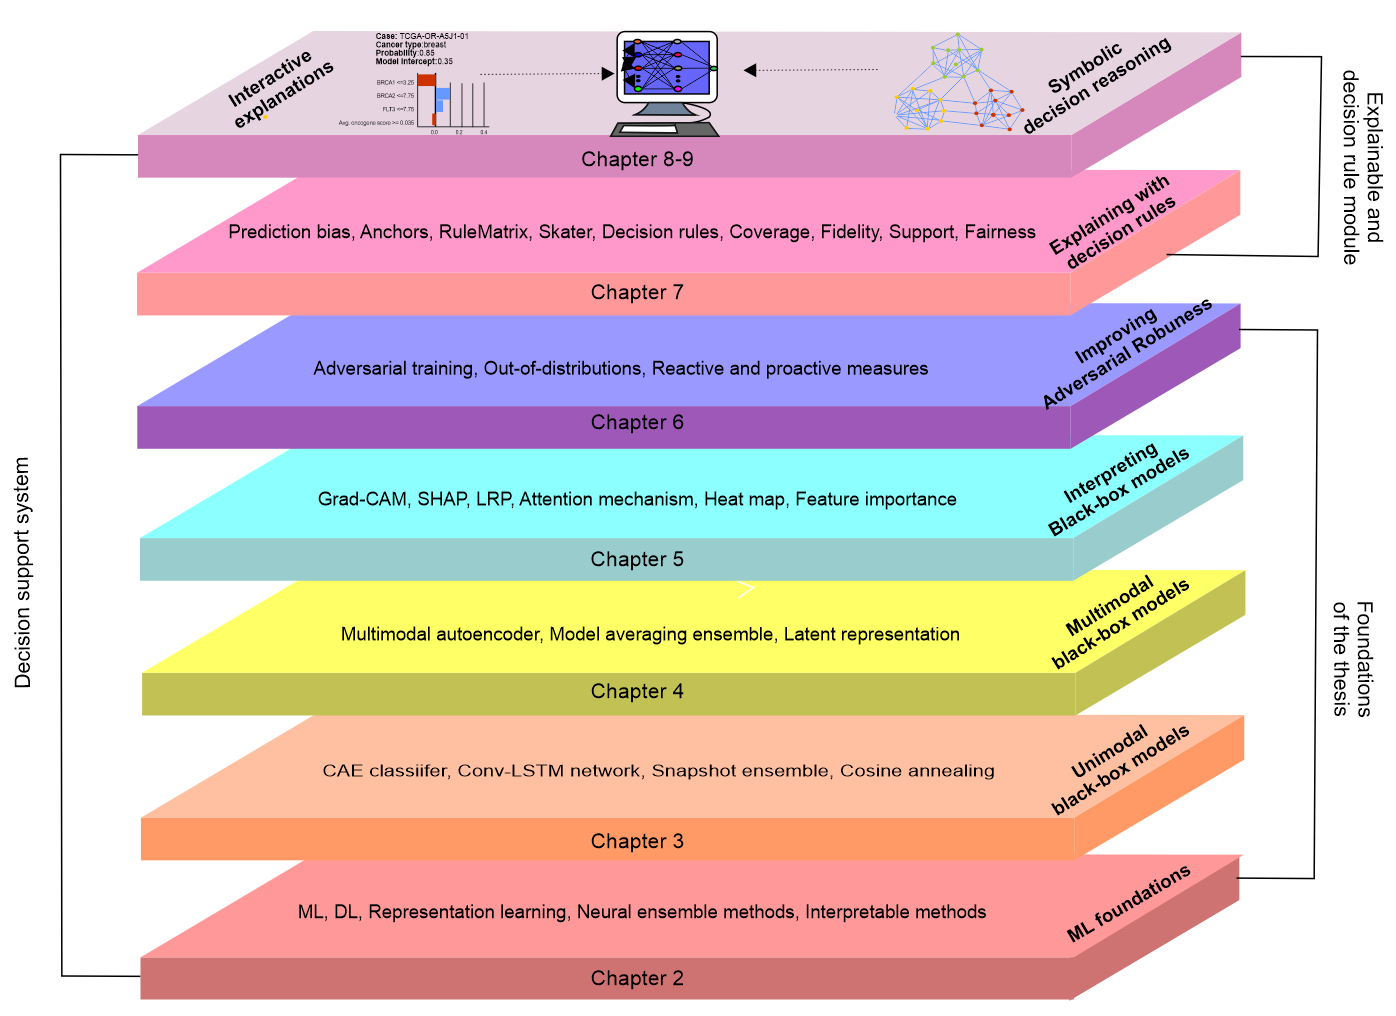
\includegraphics[scale=0.6]{images/chapter_outline.png}
		\caption{A bottom-up layout of the thesis, outlining the chapters}
        \label{fig:chapter_organization}
\end{figure*}

\section{Thesis Outline} \label{structure}
The rest of the thesis is structured into following nine chapters:  
%The brief overview of each chapter is as followed: 
\begin{enumerate}[noitemsep]
    \item \Cref{chapter:preli} provides the foundations and related concepts that will be used in the subsequent chapters. 
    \item \Cref{chapter:uni_modality} investigates the association of CNV and cancer, followed by the development of a predictive model based on single modality for the cancer type prediction task.  
    \item \Cref{chapter:multiodality}, extends the single modality based predictive model to multimodality-based by employing a multimodal neural network.  
    \item \Cref{chapter:xai} employs two different approaches to open the `black box' uni/multimodal models towards making them explainable. We identify biologically relevant biomarkers by computing their feature importance, ranking top genes across all the cancer types, and provide functional analysis.  
    \item \Cref{chapter:robustness}, is about different adversarial attacks on the models, including content moderation and out-of-distribution, followed by assessing the models' adversarial robustness. 
    \item \Cref{chapter:xai_rules} is about generating decision rules by combining model predictions and interpretations. Additionally, we identify  misclassified instances~(i.e., initial prediction by the model). 
    \item \Cref{chapter:nsr} is to perform symbolic reasoning based on a domain-specific ontology in which a reasoner decides whether a biological entity~(based on biomarkers and their attributes) is of correct types and helps to validate the findings and decision rules in order to improve human trustworthiness. 
    \item \Cref{chapter:fairness} is to improve the trustworthiness of the diagnosis by combining model interpretations, decision rules, and reasoning.
    \item \Cref{chapter:end} is to provide explanations and points out the relevance of the study, highlights its limitations, and discusses future works before concluding the dissertation. 
\end{enumerate}


